\chapter{Spectroscopie voor structuurbepaling}\label{ch:b1:structure-spectroscopy}

Een parfumeur bezorgt het laboratorium een kleurloze vloeistof die naar
ananas ruikt en vraagt wat het is. Vijftig jaar geleden zou het antwoord
weken van afbraakreacties gekost hebben. Vandaag kost het tien minuten:
een elementanalyse geeft de formule, een infraroodspectrum benoemt de
karakteristieke groep, en een spectrum van protonkernspinresonantie toont
hoe de atomen verbonden zijn. Dit hoofdstuk legt uit hoe elk spectrum
gelezen wordt --- wat licht van elk gebied met een molecuul doet, en
welke kenmerken van een spectrum welk stukje structuur dragen --- en
eindigt met dat ananasmolecuul.

\begin{recall}
Het schoolboek (jaar 11 en 12) mat \omterm{def:b1:structure-spectroscopy:absorbance}{absorbanties} met een spectrofotometer
en gebruikte de wet van Lambert-Beer om concentraties te bepalen,
identificeerde karakteristieke groepen met tabellen van infraroodbanden,
en las eenvoudige proton-NMR-spectra (aantal signalen, \omterm{def:b1:structure-spectroscopy:integration}{integratie}, de
$n + 1$-regel). Enkele, dubbele en drievoudige bindingen en de
$\pi$-binding zijn die van \cref{ch:b1:lewis-resonance-vsepr}.
\end{recall}

\section{UV-vis-spectroscopie: conjugatie en kleur}

\begin{definition}[Absorbantie en de wet van Lambert-Beer]\label{def:b1:structure-spectroscopy:absorbance}
Voor licht met intensiteit $I_0$ dat een oplossing binnenkomt en $I$ dat
haar verlaat, is de \emph{absorbantie}\index{absorbantie}
$A = \log(I_0/I)$. Voor een verdunde oplossing van één absorberend
deeltje is $A = \varepsilon\,\ell\,c$ (de wet van Lambert-Beer), waarin
$\ell$ de weglengte is, $c$ de concentratie en $\varepsilon$ de
\emph{molaire
absorptiecoëfficiënt}\index{molaire absorptiecoefficient@molaire absorptiecoëfficiënt},
een eigenschap van het deeltje bij die golflengte.
\end{definition}

Een molecuul absorbeert ultraviolet of zichtbaar licht wanneer de
energie van een foton over\-een\-komt met het verschil tussen de hoogste
bezette en de laagste lege elektronenniveaus van zijn bindingen. Voor
$\sigma$-bindingen is dat verschil groot en ligt de absorptie ver in het
ultraviolet; $\pi$-bindingen absorberen dichter bij het zichtbare, en een
keten van afwisselend dubbele en enkele bindingen absorbeert bij
langere golflengten naarmate de keten langer is.

\begin{definition}[Geconjugeerd systeem, chromofoor, absorptiemaximum]\label{def:b1:structure-spectroscopy:conjugation}
Een \emph{geconjugeerd systeem}\index{geconjugeerd systeem} is een keten
van atomen die elk een $p$-orbitaal in een $\pi$-systeem dragen, zoals
bij afwisselend dubbele en enkele bindingen (buta-1,3-dieen, benzeen). De
groep atomen die verantwoordelijk is voor een absorptie, is haar
\emph{chromofoor}\index{chromofoor}; de golflengte waarbij de \omterm{def:b1:structure-spectroscopy:absorbance}{absorbantie}
ervan het grootst is, is het
\emph{absorptiemaximum}\index{absorptiemaximum}, $\lambda_{\max}$.
\end{definition}

De niveaus van een \omterm{def:b1:structure-spectroscopy:conjugation}{geconjugeerd systeem} spreiden zich over de hele keten
uit en komen dichter bij elkaar naarmate de keten groeit, zoals de
niveaus van een deeltje in een langere doos: $\lambda_{\max}$ neemt toe
met de conjugatie. Etheen en butadieen absorberen alleen in het
ultraviolet; de elf geconjugeerde dubbele bindingen van $\beta$-caroteen
brengen de absorptie in het blauwe deel van het zichtbare. Een stof
heeft de kleur die complementair is aan het licht dat ze absorbeert:
caroteen, dat blauw en violet absorbeert, ziet er oranje uit.

\begin{omfigure}
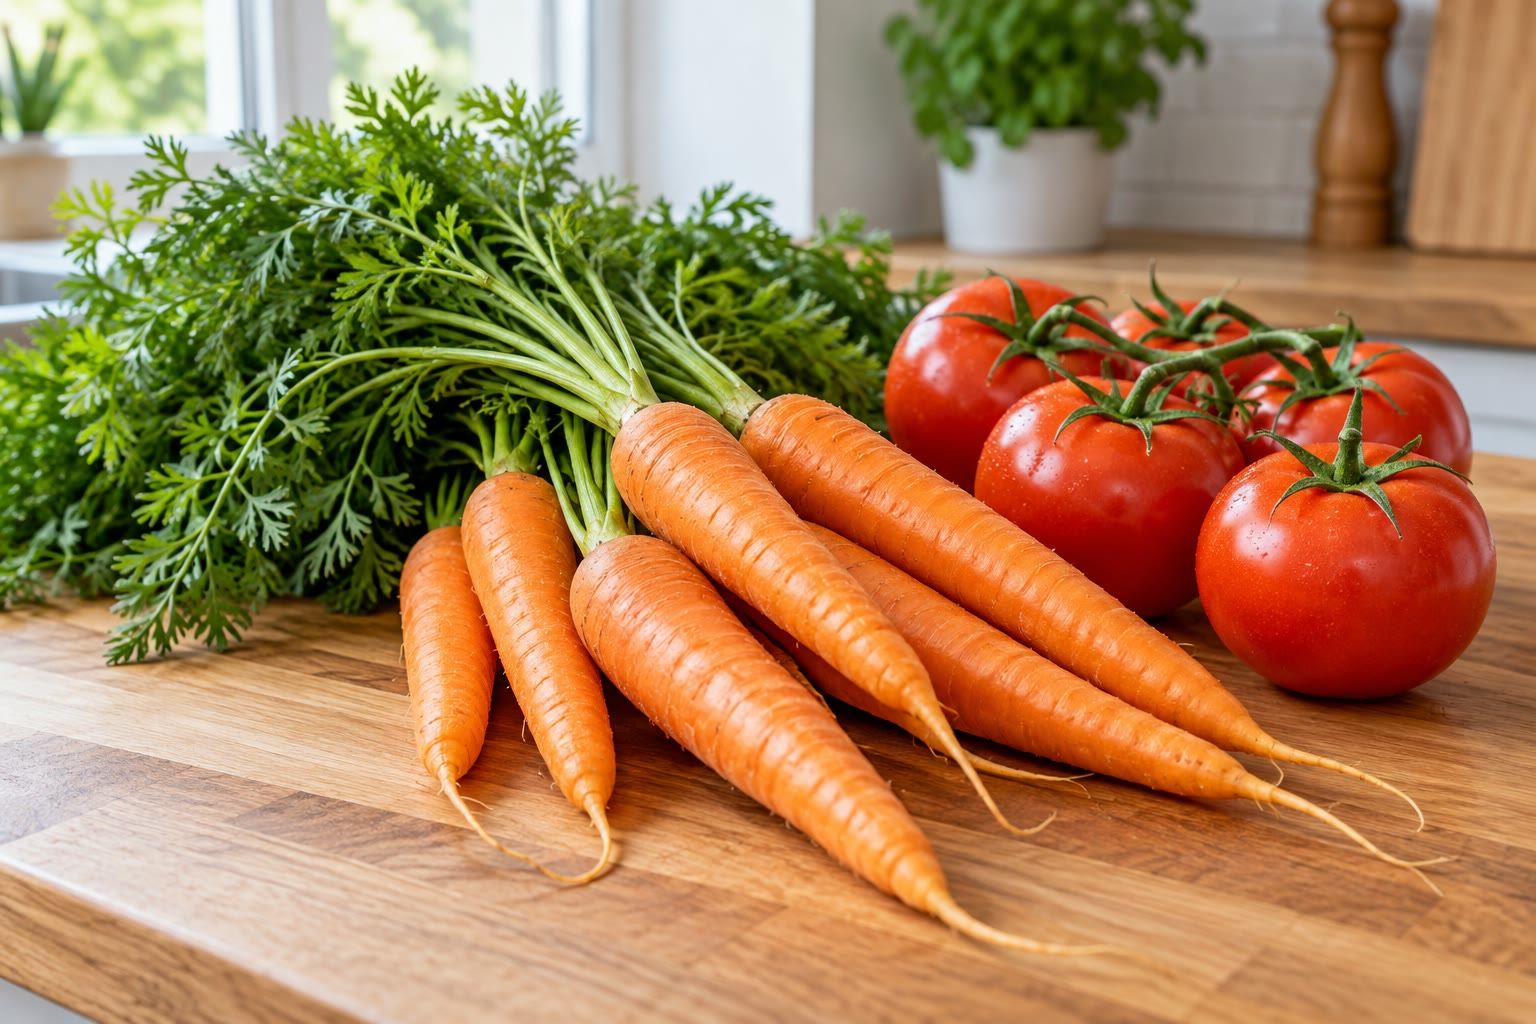
\includegraphics[width=0.55\linewidth]{images/book2/ai/b1-17-carrots-tomatoes.jpg}

{\small Wortelen en tomaten danken hun kleuren aan lange geconjugeerde
moleculen, carotenen en lycopeen, die blauw en groen licht absorberen en
oranje en rood doorlaten.}
\end{omfigure}

\begin{omfigure}
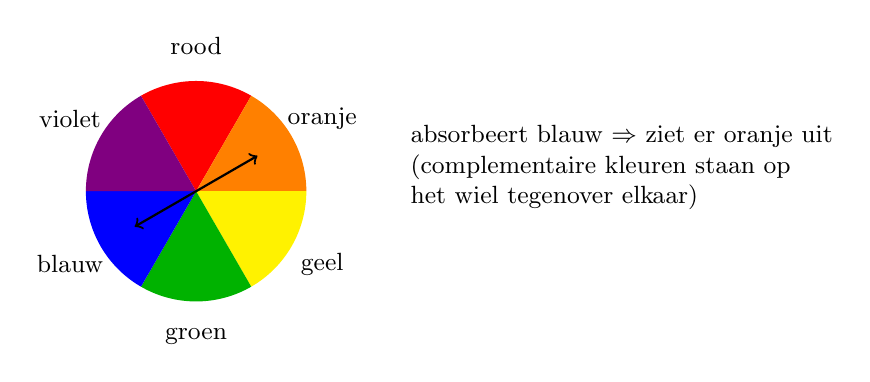
\begin{tikzpicture}[font=\small]
  \foreach \a/\c/\n in {90/red/rood, 30/orange/oranje, -30/yellow/geel, -90/green!70!black/groen, -150/blue/blauw, 150/violet/violet} {
    \fill[\c] (0,0) -- (\a-30:1.4) arc[start angle=\a-30, end angle=\a+30, radius=1.4] -- cycle;
    \node at (\a:1.85) {\n};
  }
  \draw[<->, thick] (-150:0.9) -- (30:0.9);
  \node[align=left, anchor=west] at (2.6,0.3) {absorbeert blauw $\Rightarrow$ ziet er oranje uit\\(complementaire kleuren staan op\\het wiel tegenover elkaar)};
\end{tikzpicture}

{\small Een kleurenwiel. De waargenomen kleur is het complement van de
geabsorbeerde kleur: een oplossing die in het blauw absorbeert, ziet er
oranje uit.}
\end{omfigure}

\section{Infraroodspectroscopie verdiept}

\begin{definition}[Golfgetal, transmissie, vingerafdrukgebied]\label{def:b1:structure-spectroscopy:wavenumber}
Infraroodspectra worden uitgezet tegen het
\emph{golfgetal}\index{golfgetal} $\tilde\nu = 1/\lambda$, in
\unit{cm^{-1}}, dat evenredig is met de energie van het foton. Op de
verticale as staat de \emph{transmissie}\index{transmissie}
$T = I/I_0$, in procent, zodat de banden naar beneden wijzen. Onder
ongeveer \qty{1500}{cm^{-1}} vormen veel overlappende banden, die
kenmerkend zijn voor het hele molecuul en niet voor één binding, het
\emph{vingerafdrukgebied}\index{vingerafdrukgebied}.
\end{definition}

Een binding absorbeert infrarood licht bij de frequentie waarmee ze
trilt. Zoals bij twee massa's die door een veer verbonden zijn: hoe
stijver de binding en hoe lichter de atomen, hoe hoger het \omterm{def:b1:structure-spectroscopy:wavenumber}{golfgetal}:
bindingen met waterstof (O--H, C--H) boven \qty{2800}{cm^{-1}},
drievoudige bindingen rond 2200, dubbele bindingen rond 1700--1600,
enkele bindingen tussen zwaardere atomen onder 1300. De tabel geeft
gemeten posities voor de moleculen van dit hoofdstuk, in de gasfase,
waar de moleculen geïsoleerd zijn.

\begin{omfigure}
\begin{tabular}{llr}
\hline
molecuul & binding & $\tilde\nu$ (\unit{cm^{-1}}) \\
\hline
ethanol & O--H & 3666 \\
ethanol & C--H & 2978 \\
ethanol & C--O & 1060 \\
propanon & C=O & 1738 \\
ethaanzuur & O--H & 3582 \\
ethaanzuur & C=O & 1788 \\
ethylethanoaat & C=O & 1764 \\
ethylethanoaat & C--O & 1238 \\
\hline
\end{tabular}

\smallskip
{\small Bandmaxima in infraroodspectra in de gasfase. In vloeistoffen
verbreden \omterm{def:b1:intermolecular-forces-solvents:hbond}{waterstofbruggen} de O--H-banden en verschuiven ze ze naar
lagere \omterm{def:b1:structure-spectroscopy:wavenumber}{golfgetallen}, en de C=O-banden van zuren schuiven naar beneden
wanneer het zuur paren vormt.}
% ledger: ir:ethanol-OH, ir:ethanol-CH, ir:ethanol-CO, ir:propanone-CO, ir:ethanoic-OH, ir:ethanoic-CO, ir:ethylethanoate-CO, ir:ethylethanoate-COC
\end{omfigure}

\begin{omfigure}
\begin{tikzpicture}
\begin{axis}[name=i1, width=0.86\linewidth, height=3.2cm, xmin=500, xmax=4000, x dir=reverse, ymin=0, ymax=105, ytick={0,50,100}, ylabel={$T$ (\%)}, tick label style={font=\scriptsize}, label style={font=\small}, xticklabels={}]
\addplot[omDef, thick] table[x=nu, y=T] {figdata/out/bachelor-1-spectra-ir-ethanol.dat};
\node[font=\scriptsize, anchor=west] at (axis cs:2600,25) {ethanol};
\end{axis}
\begin{axis}[name=i2, at={(i1.south)}, anchor=north, yshift=-0.25cm, width=0.86\linewidth, height=3.2cm, xmin=500, xmax=4000, x dir=reverse, ymin=0, ymax=105, ytick={0,50,100}, ylabel={$T$ (\%)}, tick label style={font=\scriptsize}, label style={font=\small}, xticklabels={}]
\addplot[omProp, thick] table[x=nu, y=T] {figdata/out/bachelor-1-spectra-ir-propanone.dat};
\node[font=\scriptsize, anchor=west] at (axis cs:2600,25) {propanon};
\end{axis}
\begin{axis}[at={(i2.south)}, anchor=north, yshift=-0.25cm, width=0.86\linewidth, height=3.2cm, xmin=500, xmax=4000, x dir=reverse, ymin=0, ymax=105, ytick={0,50,100}, ylabel={$T$ (\%)}, tick label style={font=\scriptsize}, label style={font=\small}, xlabel={golfgetal (\unit{cm^{-1}})}]
\addplot[omMeth, thick] table[x=nu, y=T] {figdata/out/bachelor-1-spectra-ir-ethanoic.dat};
\node[font=\scriptsize, anchor=west] at (axis cs:2600,25) {ethaanzuur};
\end{axis}
\end{tikzpicture}

{\small Infraroodspectra van ethanol, propanon en ethaanzuur, gesimuleerd
uit de gemeten bandposities van de tabel (hoogte en breedte van de banden
schematisch). De C=O-band rond \qty{1750}{cm^{-1}} en de O--H-band boven
\qty{3500}{cm^{-1}} onderscheiden de drie karakteristieke groepen in één
oogopslag.}
\end{omfigure}

\section{Proton-NMR: chemische verschuiving en integratie}

In een sterk magnetisch veld heeft een proton twee \omterm{def:b1:quantum-numbers:energy-level}{energieniveaus};
radiogolven met de juiste frequentie laten het van het ene naar het
andere omklappen. Die frequentie is evenredig met het magnetische veld
dat het proton werkelijk voelt, en dat wordt door de elektronen eromheen
licht verminderd. Protonen in verschillende chemische omgevingen
resoneren daarom bij licht verschillende frequenties.

\begin{definition}[Chemische verschuiving, magnetische afscherming, equivalente protonen]\label{def:b1:structure-spectroscopy:chemical-shift}
De \emph{chemische verschuiving}\index{chemische verschuiving} van een
proton is
$\delta = (\nu - \nu_{\text{ref}})/\nu_0 \times 10^6$, in \unit{ppm}, waarin
$\nu$ zijn resonantiefrequentie is, $\nu_{\text{ref}}$ die van de
protonen van tetramethylsilaan en $\nu_0$ de werkfrequentie van de
spectrometer. De verlaging van het veld bij een kern door zijn
elektronen is zijn \emph{magnetische
afscherming}\index{magnetische afscherming}: elektronenzuigende buren
(O, halogenen, C=O) ontschermen een proton en verhogen zijn $\delta$.
\emph{Equivalente protonen}\index{equivalente protonen} zijn protonen die
door een symmetrie van het molecuul of door een snelle rotatie in elkaar
overgaan; ze hebben dezelfde verschuiving.
\end{definition}

\begin{proposition}[De verschuiving hangt niet af van de spectrometer]\label{prop:b1:structure-spectroscopy:shift-field-independent}
De \omterm{def:b1:structure-spectroscopy:chemical-shift}{chemische verschuiving} van een proton is dezelfde op spectrometers met
verschillende velden.
\end{proposition}

\begin{proof}
Zowel $\nu$ als $\nu_{\text{ref}}$ zijn evenredig met het aangelegde veld
$B_0$ (elk vermenigvuldigd met zijn eigen afschermingsfactor), en dat
geldt ook voor $\nu_0$. De verhouding $(\nu - \nu_{\text{ref}})/\nu_0$ is
dus onafhankelijk van $B_0$. Verschillen in hertz daarentegen groeien met
het veld.
\end{proof}

\begin{definition}[Integratie]\label{def:b1:structure-spectroscopy:integration}
De \emph{integratie}\index{integratie} van een signaal is zijn
oppervlakte, op het spectrum afgelezen als de hoogte van een trapcurve;
de oppervlakten zijn evenredig met de aantallen protonen die de signalen
geven.
\end{definition}

\section{Spin-spinkoppeling}

\begin{definition}[Spin-spinkoppeling, koppelingsconstante, multiplet]\label{def:b1:structure-spectroscopy:coupling}
Via de bindingen verandert de magnetische toestand van een proton licht
het veld dat de protonen op de naburige koolstofatomen voelen: deze
\emph{spin-spinkoppeling}\index{spin-spinkoppeling} splitst elk signaal
in een \emph{multiplet}\index{multiplet} van lijnen die van elkaar
gescheiden zijn door de \emph{koppelingsconstante}\index{koppelingsconstante}
$J$, in hertz. Twee protonen die met elkaar koppelen, vertonen dezelfde
$J$; \omterm{def:b1:structure-spectroscopy:chemical-shift}{equivalente protonen} splitsen elkaars signaal niet.
\end{definition}

\begin{proposition}[De \texorpdfstring{$n + 1$}{n + 1}-regel]\label{prop:b1:structure-spectroscopy:n-plus-one}
Een proton (of een groep \omterm{def:b1:structure-spectroscopy:chemical-shift}{equivalente protonen}) dat met dezelfde $J$
gekoppeld is aan $n$ equivalente buren, geeft $n + 1$ lijnen, op afstand
$J$ van elkaar, met als relatieve intensiteiten de binomiaalcoëfficiënten
$\binom{n}{k}$, $k = 0$ tot
$n$ (de \emph{$n + 1$-regel}\index{n+1-regel@$n + 1$-regel}).
\end{proposition}

\begin{proof}
Elke buur bevindt zich in een van twee spintoestanden, die de
waargenomen lijn verschuiven over $+J/2$ of $-J/2$. Met $n$ buren is de
verschuiving $(k - n/2)J$, waarin $k$ het aantal buren in de eerste
toestand is: $n + 1$ waarden, op gelijke afstanden $J$. Omdat de twee
toestanden bijna even sterk bezet zijn, zijn alle $2^n$ combinaties even
waarschijnlijk, en $k$ buren in de eerste toestand komt op
$\binom{n}{k}$ manieren voor.
\end{proof}

\begin{omfigure}
\begin{tikzpicture}[font=\small, x=0.85cm, y=0.5cm]
  % quartet: three neighbours, each split +-J/2 (J = 1.5 units)
  \draw[thick] (0,4) -- (0,3.4);
  \foreach \x in {-0.75,0.75} \draw (0,3.4) -- (\x,2.4);
  \foreach \a/\b in {-0.75/-1.5, -0.75/0, 0.75/0, 0.75/1.5} \draw (\a,2.4) -- (\b,1.4);
  \foreach \a/\b in {-1.5/-2.25, -1.5/-0.75, 0/-0.75, 0/0.75, 1.5/0.75, 1.5/2.25} \draw (\a,1.4) -- (\b,0.4);
  \foreach \x/\h in {-2.25/1, -0.75/3, 0.75/3, 2.25/1} {\draw[omDef, very thick] (\x,-2.6) -- (\x,{-2.6+0.7*\h}); \draw[dotted] (\x,0.4) -- (\x,{-2.6+0.7*\h});}
  \draw (-2.8,-2.6) -- (2.8,-2.6);
  \node at (0,-3.4) {kwartet 1\,:\,3\,:\,3\,:\,1 (\ce{-CH2-} naast \ce{-CH3})};
  % triplet: two neighbours
  \begin{scope}[xshift=7.5cm]
  \draw[thick] (0,4) -- (0,3.4);
  \foreach \x in {-0.75,0.75} \draw (0,3.4) -- (\x,2.4);
  \foreach \a/\b in {-0.75/-1.5, -0.75/0, 0.75/0, 0.75/1.5} \draw (\a,2.4) -- (\b,1.4);
  \foreach \x/\h in {-1.5/1, 0/2, 1.5/1} {\draw[omProp, very thick] (\x,-2.6) -- (\x,{-2.6+0.7*\h}); \draw[dotted] (\x,1.4) -- (\x,{-2.6+0.7*\h});}
  \draw (-2.1,-2.6) -- (2.1,-2.6);
  \draw[<->] (-1.5,-0.6) -- (0,-0.6) node[midway, above, font=\scriptsize] {$J$};
  \node at (0,-3.4) {triplet 1\,:\,2\,:\,1 (\ce{-CH3} naast \ce{-CH2-})};
  \end{scope}
\end{tikzpicture}

{\small Splitsingsbomen. Elke buur splitst elke lijn in twee, op afstand
$J$; samenvallende lijnen tellen op en geven de binomiale
intensiteiten.}
\end{omfigure}

\begin{omfigure}
\begin{tikzpicture}
\begin{axis}[name=ea,
  width=0.86\linewidth, height=4.2cm, xmin=0.8, xmax=4.5, x dir=reverse, ymin=0, ymax=1.15,
  axis x line=bottom, axis y line=none, xlabel={$\delta$ (ppm)},
  tick label style={font=\scriptsize}, label style={font=\small}]
\addplot[omDef, thin] table[x=ppm, y=I] {figdata/out/bachelor-1-spectra-nmr-ethylethanoate.dat};
\node[font=\scriptsize, anchor=south] at (axis cs:4.12,0.75) {q, 2H};
\node[font=\scriptsize, anchor=west] at (axis cs:2.0,0.95) {s, 3H};
\node[font=\scriptsize, anchor=west] at (axis cs:1.15,0.8) {t, 3H};
\node[font=\small, anchor=north] at (axis cs:3.0,1.1) {\ce{CH3COOCH2CH3}};
\end{axis}
\begin{axis}[at={(ea.south)}, anchor=north, yshift=-1.3cm,
  width=0.86\linewidth, height=4.2cm, xmin=0.8, xmax=4.5, x dir=reverse, ymin=0, ymax=1.15,
  axis x line=bottom, axis y line=none, xlabel={$\delta$ (ppm)},
  tick label style={font=\scriptsize}, label style={font=\small}]
\addplot[omProp, thin] table[x=ppm, y=I] {figdata/out/bachelor-1-spectra-nmr-ethanol.dat};
\node[font=\scriptsize, anchor=south] at (axis cs:3.69,0.75) {q, 2H};
\node[font=\scriptsize, anchor=west] at (axis cs:2.55,0.6) {s, 1H};
\node[font=\scriptsize, anchor=west] at (axis cs:1.1,0.8) {t, 3H};
\node[font=\small, anchor=north] at (axis cs:2.9,1.1) {\ce{CH3CH2OH}};
\end{axis}
\end{tikzpicture}

{\small Proton-NMR-spectra van ethylethanoaat (boven) en ethanol (onder)
in \ce{CDCl3}, gesimuleerd bij \qty{90}{MHz} uit gemeten verschuivingen
en \omterm{def:b1:structure-spectroscopy:coupling}{koppelingsconstanten} ($J = \qty{7.2}{Hz}$ en \qty{7.0}{Hz}). Het
\ce{OCH2}-kwartet wordt door de zuurstof ontschermd; in ethanol koppelt
het OH-proton, dat snel tussen moleculen uitgewisseld wordt, niet, en
hangt zijn verschuiving af van de concentratie.}
% ledger: nmr:ethylethanoate-OCH2, nmr:ethylethanoate-COCH3, nmr:ethylethanoate-CH3, nmr:ethylethanoate-J, nmr:ethanol-CH2, nmr:ethanol-CH3, nmr:ethanol-OH, nmr:ethanol-J
\end{omfigure}

\begin{omfigure}
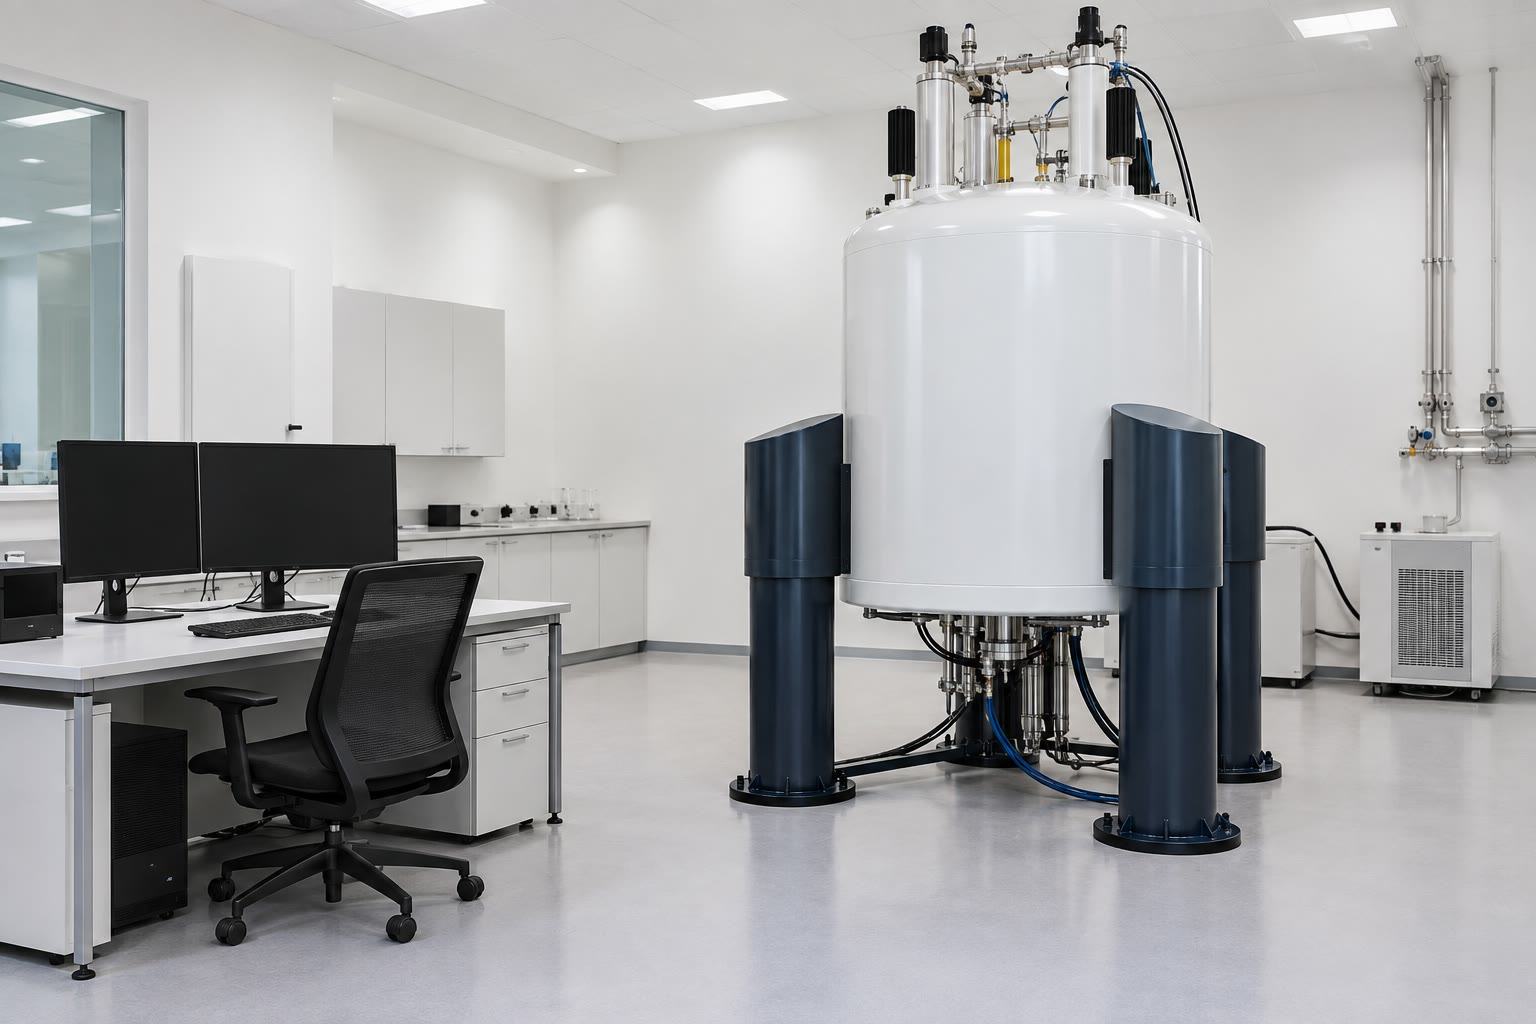
\includegraphics[width=0.5\linewidth]{images/book2/ai/b1-17-nmr.jpg}

{\small Een NMR-spectrometer: de hoge cilinder bevat een supergeleidende
magneet die door vloeibaar helium gekoeld wordt; de monsterbuis wordt in
het midden ervan neergelaten.}
\end{omfigure}

\section{Een structuur oplossen}

\begin{definition}[Onverzadigingsgraad]\label{def:b1:structure-spectroscopy:unsaturation}
De \emph{onverzadigingsgraad}\index{onverzadigingsgraad} van een formule
is het aantal ringen plus het aantal $\pi$-bindingen in het molecuul.
\end{definition}

\begin{proposition}[Onverzadigingsgraad uit de formule]\label{prop:b1:structure-spectroscopy:unsaturation-formula}
Voor een molecuul $\mathrm{C}_c\mathrm{H}_h\mathrm{N}_n\mathrm{O}_o\mathrm{X}_x$
(X een halogeen) is de \omterm{def:b1:structure-spectroscopy:unsaturation}{onverzadigingsgraad}
\[
  D = \frac{2c + 2 + n - h - x}{2} .
\]
\end{proposition}

\begin{proof}
Een open keten van $c$ koolstofatomen met alleen enkele bindingen draagt
$2c + 2$ waterstofatomen. Elke ring of $\pi$-binding neemt er twee weg.
Een tweewaardig zuurstofatoom dat in een keten ingevoegd wordt, verandert
niets; een driewaardig stikstofatoom brengt één waterstofatoom extra
mee; een halogeen neemt de plaats in van één waterstofatoom. De
ontbrekende waterstofatomen tellen en door twee delen geeft $D$.
\end{proof}

\begin{method}[Een structuur oplossen]\label{met:b1:structure-spectroscopy:solve-structure}
\begin{enumerate}
  \item Bereken $D$ uit de formule.
  \item Bepaal uit het IR-spectrum de karakteristieke groepen (C=O, O--H,
        N--H, C--O) en de afwezigheid van andere.
  \item Uit het NMR-spectrum: aantal signalen (groepen \omterm{def:b1:structure-spectroscopy:chemical-shift}{equivalente
        protonen}), \omterm{def:b1:structure-spectroscopy:integration}{integraties} (protonen per groep), verschuivingen
        (naburige groepen), multipliciteiten (aantal buren volgens de
        $n + 1$-regel), \omterm{def:b1:structure-spectroscopy:coupling}{koppelingsconstanten} (welke signalen buren zijn).
  \item Bouw fragmenten, verbind ze, en controleer elke piek aan de
        voorgestelde structuur; verwerp de isomeren die niet kloppen.
\end{enumerate}
\end{method}

\section{Oefeningen}

\begin{exercise}[$\star$]\label{exo:b1:structure-spectroscopy:1}
Een oplossing van een kleurstof van \qty{2.0e-5}{mol/L} in een cuvet van
\qty{1.00}{cm} heeft bij haar \omterm{def:b1:structure-spectroscopy:conjugation}{absorptiemaximum} een \omterm{def:b1:structure-spectroscopy:absorbance}{absorbantie} van 0.64.
Bereken $\varepsilon$, en de \omterm{def:b1:structure-spectroscopy:absorbance}{absorbantie} van een oplossing die drie keer
zo geconcentreerd is.
\end{exercise}

\begin{exercise}[$\star$]\label{exo:b1:structure-spectroscopy:2}
Bereken de \omterm{def:b1:structure-spectroscopy:unsaturation}{onverzadigingsgraad} van \ce{C6H6}, \ce{C4H8O2}, \ce{C3H7NO},
\ce{C2H3Cl} en \ce{C10H14O} (carvon). Stel voor elk één structuur voor.
\end{exercise}

\begin{exercise}[$\star$]\label{exo:b1:structure-spectroscopy:3}
Hoeveel protonsignalen, met welke \omterm{def:b1:structure-spectroscopy:integration}{integraties}, geven propanon,
ethaanzuur, 2-methylpropaan en 1,2-dichloorethaan?
\end{exercise}

\begin{exercise}[$\star$]\label{exo:b1:structure-spectroscopy:4}
Een signaal ligt op een spectrometer van \qty{400}{MHz}
\qty{1460}{Hz} van tetramethylsilaan. Wat is zijn verschuiving? Hoe ver,
in hertz, zou het bij \qty{90}{MHz} liggen? Waarom scheiden hoge velden
\omterm{def:b1:structure-spectroscopy:coupling}{multipletten} beter?
\end{exercise}

\begin{exercise}[$\star\star$]\label{exo:b1:structure-spectroscopy:5}
Voorspel de multipliciteit van elk signaal van 1-broompropaan,
\ce{CH3CH2CH2Br}, in de veronderstelling dat de \omterm{def:b1:structure-spectroscopy:coupling}{koppelingsconstanten}
gelijk zijn, en de relatieve intensiteiten van de lijnen van het
middelste signaal.
\end{exercise}

\begin{exercise}[$\star\star$]\label{exo:b1:structure-spectroscopy:6}
Hoe verschillen de IR-spectra van ethanol, propanon en ethaanzuur tussen
1700 en \qty{3700}{cm^{-1}}? Welke verbinding geeft zowel een C=O- als
een O--H-band?
\end{exercise}

\begin{exercise}[$\star\star$]\label{exo:b1:structure-spectroscopy:7}
Twee isomeren \ce{C4H8O2}: ethylethanoaat en methylpropanoaat. Voorspel
hun NMR-spectra (verschuivingen bij benadering, multipliciteiten,
\omterm{def:b1:structure-spectroscopy:integration}{integraties}) en zeg hoe je ze van elkaar onderscheidt.
\end{exercise}

\begin{exercise}[$\star\star$]\label{exo:b1:structure-spectroscopy:8}
Lees op het gesimuleerde spectrum van ethylethanoaat de afstand tussen
twee lijnen van het kwartet af in ppm en reken die om naar hertz (het
spectrum is gesimuleerd bij \qty{90}{MHz}). Vergelijk met het triplet.
\end{exercise}

\begin{exercise}[$\star\star$]\label{exo:b1:structure-spectroscopy:9}
Een verbinding \ce{C3H6O} vertoont een sterke IR-band bij
\qty{1738}{cm^{-1}} en één enkel NMR-signaal. Identificeer ze. Welk
isomeer zou een band rond \qty{2720}{cm^{-1}} en een signaal rond
\qty{9.8}{ppm} vertonen?
\end{exercise}

\begin{exercise}[$\star\star\star$]\label{exo:b1:structure-spectroscopy:10}
Bewijs de $n + 1$-regel in de vorm: een proton dat gekoppeld is aan twee
verschillende groepen buren, $n_1$ met $J_1$ en $n_2$ met $J_2$, geeft
$(n_1 +
1)(n_2 + 1)$ lijnen. Hoeveel verschillende lijnen blijven er over als
$J_1 = J_2$? Pas toe op de middelste \ce{CH2} van 1-broompropaan.
\end{exercise}

\begin{exercise}[$\star\star\star$]\label{exo:b1:structure-spectroscopy:11}
Een verbinding \ce{C4H10O} geeft geen IR-band bij 1700--1800 maar wel een
brede band rond \qty{3350}{cm^{-1}} in de vloeistof, en een NMR-spectrum
met een doublet (6H), een \omterm{def:b1:structure-spectroscopy:coupling}{multiplet} (1H), een doublet (2H) en een brede
singlet (1H). Bepaal de structuur.
\end{exercise}

\begin{exercise}[$\star\star\star$]\label{exo:b1:structure-spectroscopy:12}
Toon aan dat de \omterm{def:b1:structure-spectroscopy:absorbance}{absorbantie} van een mengsel van twee deeltjes gehoorzaamt
aan $A = \ell(\varepsilon_1c_1
+ \varepsilon_2c_2)$, en leg uit hoe metingen bij twee golflengten beide
concentraties opleveren.
\end{exercise}

\section{Probleem: het ananasmolecuul}

\begin{problem}[{Weekendprobleem --- verbrandingsanalyse en dampdichtheid,
het infraroodspectrum, het proton-NMR-spectrum, en de structuur en
molaire massa van de naar ananas ruikende ester}]
\label{pb:b1:structure-spectroscopy:1}
De onbekende stof is een vloeistof die alleen C, H en O bevat. De
verbranding van \qty{0.2500}{g} geeft \qty{0.5690}{g} koolstofdioxide en
\qty{0.2328}{g} water. Haar damp heeft een dichtheid van \qty{3.74}{g/L}
bij \qty{100}{\celsius} en \qty{1.000}{bar}. IR-banden in de gasfase:
2982, 1754, \qty{1182}{cm^{-1}} (sterk), geen boven
\qty{3100}{cm^{-1}}. Proton-NMR (\ce{CDCl3}): 4.13 (q, 2H, $J = \qty{7.2}{Hz}$),
2.28 (t, 2H), 1.66 (sextet, 2H), 1.25 (t, 3H, $J = \qty{7.2}{Hz}$), 0.95
(t, 3H) ppm. $M$: C 12.0, H 1.0, O \qty{16.0}{g/mol}; $R =
\qty{8.314}{J/(K.mol)}$.
% ledger: ir:ethylbutanoate-CH, ir:ethylbutanoate-CO, ir:ethylbutanoate-COC, nmr:ethylbutanoate-OCH2, nmr:ethylbutanoate-CH2CO, nmr:ethylbutanoate-CH2, nmr:ethylbutanoate-OCH2CH3, nmr:ethylbutanoate-CH3, nmr:ethylbutanoate-J

\begin{center}
\begin{tikzpicture}
\begin{axis}[width=0.86\linewidth, height=4.0cm, xmin=0.6, xmax=4.5, x dir=reverse, ymin=0, ymax=1.15,
  axis x line=bottom, axis y line=none, xlabel={$\delta$ (ppm)},
  tick label style={font=\scriptsize}, label style={font=\small}]
\addplot[omDef, thin] table[x=ppm, y=I] {figdata/out/bachelor-1-spectra-nmr-ethylbutanoate.dat};
\end{axis}
\end{tikzpicture}
\end{center}

\medskip
\noindent\textbf{Deel I --- De formule.}
\begin{enumerate}
  \item Bereken de massa koolstof in het monster.
  \item Bereken de massa waterstof.
  \item Leid de massa zuurstof af.
  \item Bereken de massapercentages van C, H en O.
  \item Bepaal de verhoudingsformule.
  \item Bereken uit de dampdichtheid de molaire massa (ideaal gas).
  \item Geef de molecuulformule en haar \omterm{def:b1:structure-spectroscopy:unsaturation}{onverzadigingsgraad}.
\end{enumerate}

\medskip
\noindent\textbf{Deel II --- Het infraroodspectrum.}
\begin{enumerate}[resume]
  \item Wijs de band bij \qty{1754}{cm^{-1}} toe.
  \item Wat sluit de afwezigheid van banden boven \qty{3100}{cm^{-1}} uit?
  \item Wijs de sterke band bij \qty{1182}{cm^{-1}} toe.
  \item Wijs de band bij \qty{2982}{cm^{-1}} toe.
  \item Welke familie van verbindingen blijft over, met de
        \omterm{def:b1:structure-spectroscopy:unsaturation}{onverzadigingsgraad} erbij? Waarom geen carbonzuur, geen keton met
        een ether, en geen cyclisch diol?
\end{enumerate}

\medskip
\noindent\textbf{Deel III --- Het NMR-spectrum.}
\begin{enumerate}[resume]
  \item Hoeveel groepen \omterm{def:b1:structure-spectroscopy:chemical-shift}{equivalente protonen} zijn er? Controleer de totale
        \omterm{def:b1:structure-spectroscopy:integration}{integratie}.
  \item Interpreteer het kwartet bij 4.13 ppm: buren en omgeving.
  \item Interpreteer het triplet bij 1.25 ppm. Waarom hebben de twee
        dezelfde $J$?
  \item Interpreteer het triplet bij 2.28 ppm.
  \item Interpreteer het sextet bij 1.66 ppm.
  \item Interpreteer het triplet bij 0.95 ppm.
  \item Bouw de twee fragmenten die deze signalen beschrijven.
  \item Waarom zijn de signalen bij 4.13 en 2.28 ppm het sterkst
        ontschermd?
\end{enumerate}

\medskip
\noindent\textbf{Deel IV --- De structuur.}
\begin{enumerate}[resume]
  \item Verbind de fragmenten via de estergroep: twee mogelijkheden.
        Welke is in overeenstemming met de verschuivingen?
  \item Leg uit waarom propylpropanoaat niet past.
  \item Leg uit waarom butylethanoaat niet past.
  \item Benoem de verbinding en teken haar structuur.
  \item Controleer elke IR-band en elk NMR-signaal aan de structuur.
  \item Geef de molaire massa van het ananasmolecuul.
\end{enumerate}
\end{problem}
